% This LaTeX was auto-generated from MATLAB code.
% To make changes, update the MATLAB code and export to LaTeX again.

\documentclass{article}

\usepackage[utf8]{inputenc}
\usepackage[T1]{fontenc}
\usepackage{lmodern}
\usepackage{graphicx}
\usepackage{color}
\usepackage{hyperref}
\usepackage{amsmath}
\usepackage{amsfonts}
\usepackage{epstopdf}
\usepackage[table]{xcolor}
\usepackage{matlab}

\sloppy
\epstopdfsetup{outdir=./}
\graphicspath{ {./NumericalDifferentitation_images/} }

\begin{document}

\matlabtitle{Diferenciación Numérica}

\begin{par}
\begin{flushleft}
La diferenciación númerica aproxima el valor de una de la derivada de una función utilizando una serie de puntos, la cual puede ser dada o se pueden obtener de la misma función pasada como parametro.
\end{flushleft}
\end{par}

\begin{par}
\begin{flushleft}
    En este caso usaremos la segunda opción, es decir, definiremos una función y=f(x)
\end{flushleft}
\end{par}

\begin{matlabcode}
%f = @(x) cosh(x);   % in-line function declaration
\end{matlabcode}

\begin{par}
\begin{flushleft}
El método utilizado para aproximar será el de las series de Taylor. Esto tiene como consecuencia que existan dos fuentes de error inevitables:
\end{flushleft}
\end{par}

\begin{enumerate}
\setlength{\itemsep}{-1ex}
   \item{\begin{flushleft} redondeo de la maquina (debido a la precisión limitada) \end{flushleft}}
   \item{\begin{flushleft} error de truncamiento de las series de taylor (no planeamos resolverlas hasta converger, sino truncarlas en cierto punto) \end{flushleft}}
\end{enumerate}


\matlabheading{Series de Taylor}


\vspace{1em}
\begin{par}
\begin{flushleft}
Por definición, la aproximación con una serie de taylor par auna función $f(x)$\textit{ }alderedor del punto $a$ es:
\end{flushleft}
\end{par}

\begin{par}
$$f\left(x\right)\;\approx f\left(a\right)+\frac{f^{\prime } \left(a\right)}{1!}\left(x-a\right)+\frac{f^{\prime \prime } \left(a\right)}{2!}{\left(x-a\right)}^2 +\ldotp \ldotp \ldotp ,=\sum_{n=0}^{\infty } \frac{f^{\left(n\right)} \left(a\right)}{n!}{\left(x-a\right)}^n$$
\end{par}

\begin{par}
\begin{flushleft}
Ahora, si aproximamos en funcion de $x+h$ alrededor de un punto $x$
\end{flushleft}
\end{par}

\begin{par}
$$f\left(x+h\right)\approx f\left(x\right)+\frac{f^{\prime } \left(x\right)}{1!}\left(h\right)+\frac{f^{\prime \prime } \left(x\right)}{2!}{\left(h\right)}^2 +\ldotp \ldotp \ldotp ,=\sum_{n=0}^{\infty } \frac{f^{\left(n\right)} \left(x\right)}{n!}{\left(h\right)}^n$$
\end{par}

\matlabheading{Primera derivada}


\vspace{1em}
\begin{par}
\begin{flushleft}
Resolviendo varias funciones de taylor, podemos despejar la primera derivada de x de la ecuacion resultante al substraer de la serie de f(x+h) alrededor de x de la serie de f(x-h) alrededor de x.
\end{flushleft}
\end{par}

\begin{par}
$$f\left(x+h\right)-f\left(x-h\right)\approx 2\left\lbrack {\textrm{hf}}^{\prime } \left(x\right)+\frac{h^3 }{3!}f^{\prime \prime \prime } \left(x\right)+\ldotp \ldotp \ldotp ,\right\rbrack$$
\end{par}

\begin{par}
\begin{flushleft}
despejando para $f^{\prime } (x)$
\end{flushleft}
\end{par}

\begin{par}
$$f^{\prime } \left(x\right)\approx \frac{f\left(x+h\right)-f\left(x-h\right)}{2h}-\frac{1}{h}\left(\frac{h^3 }{3!}{{f^{\prime } }^{\prime } }^{\prime } \left(x\right)+\ldotp \ldotp \ldotp ,\right)\approx \frac{f\left(x+h\right)-f\left(x-h\right)}{2h}-\frac{h^2 }{6}{{f^{\prime } }^{\prime } }^{\prime } \left(x\right)-\ldotp \ldotp \ldotp$$
\end{par}

\begin{par}
\begin{flushleft}
por lo que si fijamos x y variamos h para identificar la precision de la aproximación, podemos asumir que el error de truncamiento se comporta como $h^2$. Es decir,
\end{flushleft}
\end{par}

\begin{par}
\begin{center}
$f^{\prime } \left(x\right)\approx \frac{f\left(x+h\right)-f\left(x-h\right)}{2h}$$+\mathcal{O}(h^2 )$.
\end{center}
\end{par}

\begin{par}
\begin{flushleft}
Ya que \textit{h }es la mayoria de las veces menor a 1, a mayor grado de exponente en \textit{h}, mejor es la aproximación.
\end{flushleft}
\end{par}

\begin{par}
\begin{flushleft}
En el caso de querer mejorar la precisión, deberiamos calcular más series de Taylor como funciones de $x\pm (n)h$ y cancelaras entre sí.
\end{flushleft}
\end{par}

\matlabheading{Generalización}


\vspace{1em}
\begin{par}
\begin{flushleft}
Usando el método anteriormente descrito, llegamos a tres formas distintas, las aproximaciones centradas, hacia adelante y hacia atrás. Analizaremos la primera y la segunda derivada de las funciones $f(x)=e^{-x}$  y $g(x)=\ln x$
\end{flushleft}
\end{par}

\begin{matlabcode}
format long
syms g(x) f(x);
f(x)=exp(-x) 
\end{matlabcode}
\begin{matlabsymbolicoutput}
f(x) = 

\hskip1em $\displaystyle {\mathrm{e}}^{-x} $
\end{matlabsymbolicoutput}
\begin{matlabcode}
func1 = matlabFunction(f(x))
\end{matlabcode}
\begin{matlaboutput}
func1 = 
    @(x)exp(-x)

\end{matlaboutput}
\begin{matlabcode}
%f(x)=log(x)
%func2 = @(x) log(x);

c=0.6;
i = 1:50;
arr = @(x) double(power(c,x));

hs = arr(i)
\end{matlabcode}
\begin{matlaboutput}
hs = 1x50    
   0.600000000000000   0.360000000000000   0.216000000000000   0.129600000000000   0.077760000000000   0.046656000000000   0.027993600000000   0.016796160000000   0.010077696000000   0.006046617600000   0.003627970560000   0.002176782336000   0.001306069401600   0.000783641640960   0.000470184984576   0.000282110990746   0.000169266594447   0.000101559956668   0.000060935974001   0.000036561584401   0.000021936950640   0.000013162170384   0.000007897302231   0.000004738381338   0.000002843028803   0.000001705817282   0.000001023490369   0.000000614094221   0.000000368456533   0.000000221073920   0.000000132644352   0.000000079586611   0.000000047751967   0.000000028651180   0.000000017190708   0.000000010314425   0.000000006188655   0.000000003713193   0.000000002227916   0.000000001336749   0.000000000802050   0.000000000481230   0.000000000288738   0.000000000173243   0.000000000103946   0.000000000062367   0.000000000037420   0.000000000022452   0.000000000013471   0.000000000008083

\end{matlaboutput}
\begin{matlabcode}
x=2
\end{matlabcode}
\begin{matlaboutput}
x = 
     2

\end{matlaboutput}
\begin{matlabcode}

\end{matlabcode}


\matlabheading{Diferencia Central Finita}


\vspace{1em}
\begin{par}
\begin{flushleft}
Las aproximaciones pueden realizarse de forma "centralizada", este nombre proviene de la necesidad de calcular los puntos $f\left(x+h\right)$ y $f\left(x-h\right)$ para una x que se encuentra en el centro de estos dos. 
\end{flushleft}
\end{par}

\begin{par}
\begin{flushleft}
    Usaremos las dos siguientes formulas para aproximar la primera y segunda derivada de las funciones.
\end{flushleft}
\end{par}

\begin{par}
$$f^{\prime } \left(x\right)\approx \frac{f\left(x+h\right)-f\left(x-h\right)}{2h}$$$$+\mathcal{O}(h^2 )$$
\end{par}

\begin{par}
$$f^{\prime \prime } \left(x\right)\approx \frac{f\left(x+h\right)-2f\left(x\right)+f\left(x-h\right)}{h^2 }$$$$+\mathcal{O}(h^2 )$$
\end{par}

\begin{matlabcode}
%calcular valor real
df      = diff(f)              %Primer derivada 
\end{matlabcode}
\begin{matlabsymbolicoutput}
df(x) = 

\hskip1em $\displaystyle -{\mathrm{e}}^{-x} $
\end{matlabsymbolicoutput}
\begin{matlabcode}
dfX    = double(df(x))
\end{matlabcode}
\begin{matlaboutput}
dfX = 
  -0.135335283236613

\end{matlaboutput}
\begin{matlabcode}
d2f     = diff(f,2)            %Segunda derivada
\end{matlabcode}
\begin{matlabsymbolicoutput}
d2f(x) = 

\hskip1em $\displaystyle {\mathrm{e}}^{-x} $
\end{matlabsymbolicoutput}
\begin{matlabcode}
df2X   = double(d2f(x))
\end{matlabcode}
\begin{matlaboutput}
df2X = 
   0.135335283236613

\end{matlaboutput}
\begin{matlabcode}

error           = zeros([10,length(hs)]);
approximations  = zeros([1,10]);

j=1;
for h = hs
    approximations(1) = firstCenteredDerivative(func1,x,h);     %centered first derivative - h^2
    approximations(2) = secondCenteredDerivative(func1,x,h);    %centered second derivative - h^2
    approximations(3) = forwardFiniteDifference(func1,x,h,1,1); %forward Finite first derivative -h
    approximations(4) = forwardFiniteDifference(func1,x,h,1,2); %forward Finite first derivative -h^2
    approximations(5) = forwardFiniteDifference(func1,x,h,2,1); %forward Finite second derivative -h
    approximations(6) = forwardFiniteDifference(func1,x,h,2,2); %forward Finite second derivative -h^2
    approximations(7) = backwardFiniteDifference(func1,x,h,1,1);%backward Finite first derivative -h
    approximations(8) = backwardFiniteDifference(func1,x,h,1,2);%backward Finite first derivative -h^2
    approximations(9) = backwardFiniteDifference(func1,x,h,2,1);%backward Finite second derivative -h
    approximations(10)= backwardFiniteDifference(func1,x,h,2,2);%backward Finite second derivative -h^2
    error(1,j)=abs(approximations(1)/dfX -1);
    error(2,j)=abs(approximations(2)/df2X -1);
    error(3,j)=abs(approximations(3)/dfX -1);
    error(4,j)=abs(approximations(4)/dfX -1);
    error(5,j)=abs(approximations(5)/df2X -1);
    error(6,j)=abs(approximations(6)/df2X -1);
    error(7,j)=abs(approximations(7)/dfX -1);
    error(8,j)=abs(approximations(8)/dfX -1);
    error(9,j)=abs(approximations(9)/df2X -1);
    error(10,j)=abs(approximations(10)/df2X -1);
    j = j+1;
end


figure;
loglog(hs,error(1,:),'r-*')
hold on
[minV,idx] = min(error(1,:));
loglog(hs(idx),error(1,idx),"r o",'MarkerSize',7,'LineWidth',3)
set(gca,'XDir','reverse')
xlabel("h (step size)")
ylabel("Relative Error (%)")
grid
title("Error vs size of h for central finite difference of first derivative")
legend("f^{(1)}(x) +O(h^2)","min error")
hold off
\end{matlabcode}
\begin{center}
\includegraphics[width=\maxwidth{56.196688409433015em}]{figure_0.eps}
\end{center}
\begin{matlabcode}

figure;
loglog(hs,error(2,:),'r-*')
hold on;
[minV,idx] = min(error(2,:));
loglog(hs(idx),error(2,idx),"r o",'MarkerSize',7,'LineWidth',3)
set(gca,'XDir','reverse')
xlabel("h (step size)")
ylabel("Relative Error (%)")
grid
title("Error vs length of h for central finite difference of second derivative")
legend("f^{(2)}(x) +O(h^2)","min error")
hold off
\end{matlabcode}
\begin{center}
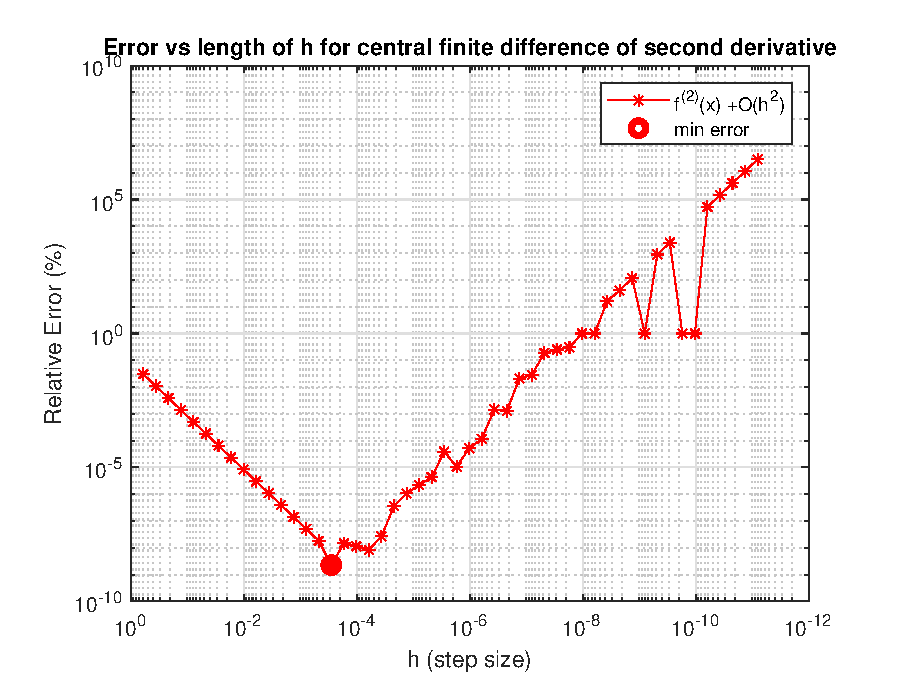
\includegraphics[width=\maxwidth{56.196688409433015em}]{figure_1.eps}
\end{center}
\begin{matlabcode}

\end{matlabcode}


\matlabheading{Diferencia finita hacia adelante }


\vspace{1em}
\begin{par}
\begin{flushleft}
Similarmente a como despejamos la primera y segunda derivada de un sistema de ecuaciones de series de Taylor, podemos despejarlas de manera que sólo usemos puntos adelante de $x$, es decir, puntos de la forma $x+\left(n\right)h$ para $n\ge 0$.
\end{flushleft}
\end{par}

\matlabheadingtwo{Primer derivada finita hacia adelante}


\vspace{1em}
\begin{par}
\begin{center}
$f^{\prime } \left(x\right)\approx \frac{f\left(x+h\right)-f\left(x\right)}{h}+$$\mathcal{O}(h)$                                             (a)
\end{center}
\end{par}

\begin{par}
\begin{center}
$f^{\prime } \left(x\right)\approx \frac{-\frac{1}{2}\;f\left(x+2h\right)+2f\left(x+h\right)-\frac{3}{2}f\left(x\right)}{h}+$$\mathcal{O}(h^2 )$             (b)
\end{center}
\end{par}

\begin{par}
\begin{flushleft}
La ecuación (a) y (b) aproximan la primera derivada de $f\left(x\right)$, sin embargo (b) lo hace con mayor precisión, pues el error de truncamiento es de orden 2, y como $h\le 1\;$, el error se minimiza.
\end{flushleft}
\end{par}

\begin{matlabcode}

figure;
loglog(hs,error(3:4,:),"-*")
hold on
[minV,idx] = min(error(3,:));
loglog(hs(idx),error(3,idx),"b o",'MarkerSize',7,'LineWidth',3)
[minV,idx] = min(error(4,:));
loglog(hs(idx),error(4,idx),"r o",'MarkerSize',7,'LineWidth',3)
set(gca,'XDir','reverse')
grid
xlabel("h (step size)")
ylabel("Relative Error (%)")
title("Error vs length of h for Forward Finite Difference of first derivative")
legend("f^{(1)}(x) +O(h)","f^{(1)}(x) +O(h^2)","min error f'","min error f''" )
hold off
\end{matlabcode}
\begin{center}
\includegraphics[width=\maxwidth{56.196688409433015em}]{figure_2.eps}
\end{center}


\matlabheadingtwo{Segunda derivada finita hacia adelante}


\vspace{1em}
\begin{par}
\begin{center}
${f^{\prime } }^{\prime } \left(x\right)\approx \;\frac{f\left(x+2h\right)-2f\left(x+h\right)+f\left(x\right)}{h^2 }+$$\mathcal{O}(h)$                                                  (a)
\end{center}
\end{par}

\begin{par}
\begin{center}
${f^{\prime } }^{\prime } \left(x\right)\approx \;\frac{-f\left(x+3h\right)+4f\left(x+2h\right)-5f\left(x+h\right)+2f\left(x\right)}{h^2 }+$$\mathcal{O}(h^2 )$                        (b)
\end{center}
\end{par}

\begin{par}
\begin{flushleft}
Al igual que con la primera derivada finita hacia adelante, la ecuación (b) aproxima a la segunda con mayor presición que la ecuación (a).
\end{flushleft}
\end{par}

\begin{matlabcode}

%error

figure;
loglog(hs,error(5:6,:),"-*")
hold on
[minV,idx] = min(error(5,:));
loglog(hs(idx),error(5,idx),"b o",'MarkerSize',7,'LineWidth',3)
[minV,idx] = min(error(6,:));
loglog(hs(idx),error(6,idx),"r o",'MarkerSize',7,'LineWidth',3)
set(gca,'XDir','reverse')
xlabel("h (step size)")
ylabel("Relative Error (%)")
title("Error vs length of h for Forward Finite Difference of second derivative")
legend("f^{(2)}(x) +O(h)","f^{(2)}(x) +O(h^2)","min error f'","min error f''" )
grid
hold off
\end{matlabcode}
\begin{center}
\includegraphics[width=\maxwidth{56.196688409433015em}]{figure_3.eps}
\end{center}


\matlabheading{Diferencia finita hacia atrás}


\vspace{1em}
\begin{par}
\begin{flushleft}
Para la diferencia finita hacia atrás usamos la función valuada en $x$ y $x-h$, es decir, en lugar de los valores de $x$ y $x+h$ tenemos: $f\left(x\right)-f\left(x-h\right)$.
\end{flushleft}
\end{par}

\matlabheadingtwo{Primera derivada finita hacia atrás}

\begin{par}
\begin{flushleft}
A continuación hay dos fórmulas para la primera derivada hacia atrás. La segunda (b) es más precisa pues para su elaboración se incorporan más términos de la serie de Taylor. 
\end{flushleft}
\end{par}

\begin{par}
\begin{center}
$f^{\prime } \left(x\right)=\;\frac{f\left(x\right)-f\left(x-h\right)}{h}+$$\mathcal{O}(h)$                                              (a)
\end{center}
\end{par}

\begin{par}
\begin{center}
$f^{\prime } \left(x\right)=\frac{3f\left(x\right)-4f\left(x-h\right)+f\left(x-2h\right)}{2h}+$$\mathcal{O}(h^2 )$                      (b)
\end{center}
\end{par}


\vspace{1em}
\begin{matlabcode}

figure;
loglog(hs,error(7:8,:),"-*")
hold on
[minV,idx] = min(error(7,:));
loglog(hs(idx),error(7,idx),"b o",'MarkerSize',7,'LineWidth',3)
[minV,idx] = min(error(8,:));
loglog(hs(idx),error(8,idx),"r o",'MarkerSize',7,'LineWidth',3)
set(gca,'XDir','reverse')
grid
xlabel("h (step size)")
ylabel("Relative Error (%)")
title("Error vs length of h for Backward Finite Difference of first derivative")
legend("f^{(1)}(x) +O(h)","f^{(1)}(x) +O(h^2)","min error f'","min error f''" )
hold off
\end{matlabcode}
\begin{center}
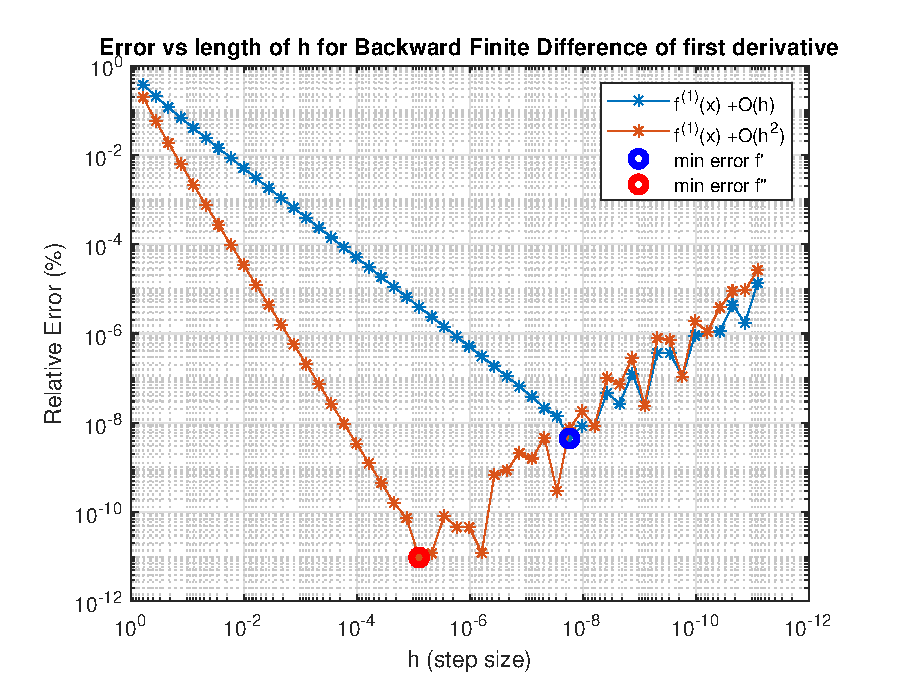
\includegraphics[width=\maxwidth{56.196688409433015em}]{figure_4.eps}
\end{center}

\vspace{1em}

\matlabheadingthree{Segunda derivada finita hacia atrás }

\begin{par}
\begin{flushleft}
De la misma manera que para la primer derivada finita hacia atrás, la segunda fórmula (b) es más precisa que la primera (a).
\end{flushleft}
\end{par}


\vspace{1em}
\begin{par}
\begin{center}
${f^{\prime } }^{\prime } \left(x\right)=\frac{f\left(x\right)-2f\left(x-h\right)+f\left(x-2h\right)}{h^2 }+$$\mathcal{O}(h)$                                         (a)
\end{center}
\end{par}

\begin{par}
\begin{center}
${f^{\prime } }^{\prime } \left(x\right)=\frac{2f\left(x\right)-5f\left(x-h\right)+4f\left(x-2h\right)-f\left(x-3h\right)}{\;h^2 }+$$\mathcal{O}(h^2 )$                (b)
\end{center}
\end{par}


\vspace{1em}
\begin{matlabcode}

figure;
loglog(hs,error(9:10,:),"-*")
hold on
[minV,idx] = min(error(9,:));
loglog(hs(idx),error(9,idx),"b o",'MarkerSize',7,'LineWidth',3)
[minV,idx] = min(error(10,:));
loglog(hs(idx),error(10,idx),"r o",'MarkerSize',7,'LineWidth',3)
set(gca,'XDir','reverse')
grid
xlabel("h (step size)")
ylabel("Relative Error (%)")
title("Error vs length of h for Backward Finite Difference of second derivative")
legend("f^{(2)}(x) +O(h)","f^{(2)}(x) +O(h^2)","min error f'","min error f''" )
hold off
\end{matlabcode}
\begin{center}
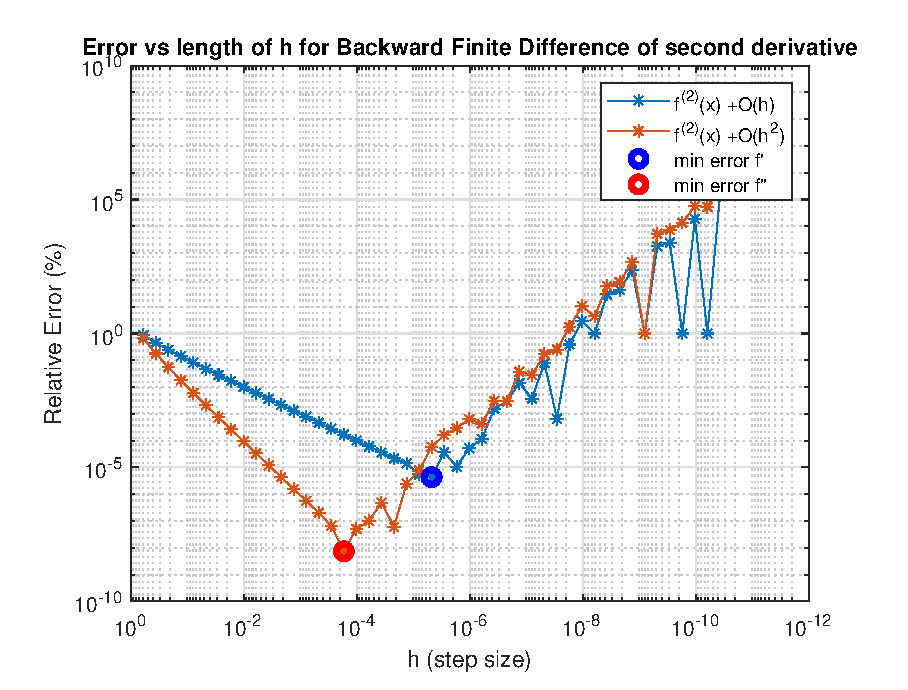
\includegraphics[width=\maxwidth{56.196688409433015em}]{figure_5.eps}
\end{center}


\matlabheading{m-th derivative with precision n }

\begin{matlabcode}
n=4;m=2;
NumCoefs=2*floor((m+1)/2)-1+n; p=(NumCoefs-1)/2;
% Solve system A*w = b
A=power(-p:p,(0:2*p)'); b=zeros(2*p+1,1); b(m+1)=factorial(m); coefs=A\b %inv(A)*b
\end{matlabcode}
\begin{matlaboutput}
coefs = 5x1    
  -0.083333333333333
   1.333333333333333
  -2.500000000000000
   1.333333333333333
  -0.083333333333333

\end{matlaboutput}
\begin{matlabcode}

% Round elements near values close to machine-epsilon to zero
coefs = coefs.*not(abs(coefs)<2000*eps);
format rational;
coefs
\end{matlabcode}
\begin{matlaboutput}
coefs = 
      -1/12    
       4/3     
      -5/2     
       4/3     
      -1/12    

\end{matlaboutput}

\end{document}
